% !TeX encoding = windows-1251
\documentclass[a4paper,12pt]{article}
\usepackage{newlistok}
\usepackage{tikz}

\УвеличитьВысоту{2.3cm}
\УвеличитьШирину{1.5cm}
\renewcommand{\spacer}{\vspace{1mm}}

\Заголовок{Домашняя работа}
\def\словоЛисток{ДЗ \No\/}
\НомерЛистка{2}
\ДатаЛистка{20 февраля 2013г.}

\begin{document}

%\ncopy{1}{
\vspace*{-17mm}
\СоздатьЗаголовок
\задача
Придумайте такое отображение $f\colon \R \to \R$, что у каждой точки\\
\пункт
ровно 1 прообраз;
\пункт
ровно 2 или 3 прообраза.
\кзадача

\УстановитьГраницы{0mm}{30mm}
\задача
Верно ли, что для любых множеств $A$, $B$, $C$ и $D$ верно равенство:\\
$((A\setminus B)\setminus C) \cap D = (D\setminus B) \cap (A\setminus C)$?
\кзадача

\задача
\onlyput{15cm}{-1.1cm}{
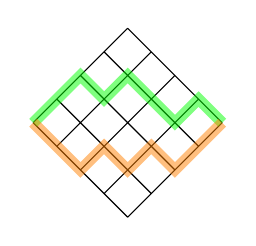
\begin{tikzpicture}[scale=.3]
\pgftransformcm{1}{-1}{1}{1}{(0,0)}
\draw [step=1] grid (4,4);
\draw[line width=4pt,green,opacity=.5] (0,0) -- (0,2) -- (1,2) -- (1,3) -- (3,3) -- (3,4) -- (4,4);
\draw[line width=4pt,orange,opacity=.5] (0,0) -- (2,0) -- (2,1) -- (3,1) -- (3,2) -- (4,2) -- (4,4);
\end{tikzpicture}}%
\onlyput{14.8cm}{-1.5cm}{ \hbox{$(()())()$; $(((())))$} }%
Чего больше: путей из точки $(0,0)$ в точку $(2n,0)$ с шагами \лк направо вверх\пк и \лк направо вниз\пк (то есть $(1,1)$ и $(1,-1)$) или число способов расставить $n$ открывающих и $n$ закрывающих скобок так, чтобы выражение было корректно (то есть число открывающих скобок на каждом шагу было не меньше числа закрывающих).
\кзадача
\ВосстановитьГраницы
\hrl
{\small Для получения оценки $n$ необходимо правильно решить $n-1$ задачу.}
%}

\bigskip
\noindent%
\onlyput{-\oddsidemargin}{-300mm}{%

\begin{tikzpicture}[scale=.5]
\draw[step=1,opacity=.5,color=gray] grid (42,60);
\end{tikzpicture}}%
\newpage
\vspace*{-\topmargin}\vspace*{-22mm}%
\noindent%
\onlyput{-\oddsidemargin}{-300mm}{%

\begin{tikzpicture}[scale=.5]
\draw[step=1,opacity=.5,color=gray] grid (42,60);
\end{tikzpicture}}%


\end{document}
